%---------------------------------------------------------------------------
\svnidlong 
{$HeadURL: https://svn.fil.univ-lille1.fr/svn/sedoglav_PDC/trunk/Cours/06/06.tex $} 
{$LastChangedDate: 2011-10-17 10:28:35 +0200 (Mon, 17 Oct 2011) $} 
{$LastChangedRevision: 61 $} 
{$LastChangedBy: sedoglav $} 
\svnid{$Id: 06.tex 61 2011-10-17 08:28:35Z sedoglav $} 
%------------------------------------------------------------------------------
%  \slideheading{Plan de la s\'eance}%
%  \begin{enumerate}
%  \item Compl\'ements sur les pointeurs 
%    \begin{enumerate}
%    \item Pointeurs de fonctions
%    \item D\'eclarations complexes
%    \end{enumerate}
%  \item[]
%  \item Les arguments de la fonction main
%  \item[]
%  \item Allocation dynamique
%  \end{enumerate}    
%------------------------------------------------------------------------------
\section{Allocation dynamique}
\begin{frame}
  \frametitle{malloc et free}%
  Ces fonctions n\'ecessitent l'inclusion de l'ent\^ete stdlib.h et
  manipulent un segment de m\'emoire  --- appel\'e
  le tas --- associ\'e au processus.
  \par\smallskip
  Fonction d'allocation dynamique de m\'emoire~:
  \begin{itemize}
  \item fonction {\tt malloc} de la librairie standard~;
  \item r\'eserve un espace m\'emoire dans le tas du processus~;
    \begin{itemize}
    \item  {\tt void *malloc(size\_t size)}\\
      r\'eserve {\tt size} octets dans le tas et retourne un pointeur 
      sur la zone allou\'ee ({\tt NULL} en cas d'echec).
    \end{itemize}
  \end{itemize}
  Fonction de d\'esallocation de m\'emoire~;
  \begin{itemize}
  \item fonction {\tt free} de la librairie standard~;
    \begin{itemize}
     \item  {\tt void free(void *ptr)}\\
      lib\`ere une zone allou\'ee par un pr\'ec\'edent {\tt malloc}. \\
      {\tt ptr} doit obligatoirement \^etre un pointeur retourn\'e par
      un pr\'ec\'edent {\tt malloc}.
    \end{itemize}
  \end{itemize}
\end{frame}
%------------------------------------------------------------------------------
\begin{frame}[fragile]
  \frametitle{Conversion de type} 
  Petit rappel sur le for\c{c}age de type~: coercition (cast)
  \begin{itemize}
  \item force la conversion de type de la valeur d'un expression~:\\
    \centerline{{\tt (}\;{\it type}\;{\tt)}\; {\it expression}}
  \item ne peut \^etre une valeur gauche.
  \end{itemize}
  
  Petit rappel sur la taille d'un objet~: op\'erateur
  {\tt sizeof}
  \begin{itemize}
  \item  {\tt sizeof({\it identificateur\_de\_type})}\\
    donne la taille en octets de tout objet de type
    {\it identificateur\_de\_type}~;
  \item Avec beaucoup de pr\'ecaution, on peut utiliser \\
    {\tt sizeof {\it expression}}\\
    qui donne la taille en octets de son op\'erande {\tt expression}.
    Mais attention~:
\begin{verbatim}
char *ch = "Hello world" ; /*comment est-ce stock\'e~?*/ 
int main(void){
  char *chlocal = "Hello world" ; /* idem */
  return sizeof(ch) ; /* que retourne cette fonction~?*/
}
\end{verbatim}
  \end{itemize}
\end{frame}
%------------------------------------------------------------------------------
\begin{frame}[fragile]
  Exemple lors de l'allocation dynamique~:
\begin{verbatim}
#include <stdlib.h>
struct point {
  int x, y;
};

struct point * reserve_n_points (int n){
  return (struct point *) malloc(sizeof(struct point)*n);
}

int main(void){
  struct point *p_point = reserve_n_points(10) ;
  return 0 ;
}
\end{verbatim}

  \textbf{Attention~:} l'espace m\'emoire allou\'e dynamiquement sur ---
  le tas --- dans
  une fonction n'est pas d\'etruit en fin de fonction comme l'espace
  associ\'e \`a une variable automatique (locale).
  
  \index{Allocation dynamique}
  \index{\verb?malloc?}
  \index{\verb?free?}
  \index{Coercition (cast)}
  \index{Forcage de type}
  \index{Op\'erateur!taille d'un objet}
  \index{\verb?sizeof?}
  
\end{frame}
%------------------------------------------------------------------------------
\section{Les pointeurs de fonctions}
%------------------------------------------------------------------------------
\begin{frame} 
  \frametitle{Remarques sur les fonctions en~C}
  Une fonction en C est 
  \begin{itemize}
  \item un objet de premi\`ere classe~: directement manipulable~;
  \item avec un d\'eclarateur postfixe {\tt ()}~: {\tt int sqr(int);}
  \item son fonctionnement est analogue \`a celui des tableaux~:
  \end{itemize}
    \par\bigskip
    \begin{center}
      \begin{tabular}[h]{l|l}
        D\'eclaration d'un tableau & D\'eclaration d'une fonction \\
        de 5 entiers & enti\`ere \`a valeur enti\`ere \\
        {\tt int ar[5];} & {\tt int sqr(int x);} \\
        {\tt temp = ar[i];} & {\tt temp = sqr(i);} \\
        d\'er\'ef\'erencement du pointeur & d\'er\'ef\'erencement du pointeur \\
        d'entiers {\tt ar} et acc\`es & de fonction {\tt sqr} et appel \\
        \`a son \'el\'ement {\tt i}. & avec le param\`etre {\tt i}.
      \end{tabular}
    \end{center}
\end{frame}
%------------------------------------------------------------------------------
\begin{frame}[fragile]
 \textbf{L'identificateur d'une fonction en C est associ\'e \`a un pointeur de
    fonction constant qui pointe sur elle m\^eme.}
  \par\smallskip
  Plus pr\'ecis\'ement, le nom d'une fonction est un pointeur de
  fonction {\tt constant} sur le d\'ebut du code correspondant \`a
  cette fonction.
\begin{verbatim}
int                      .text                         
foo                      .globl foo .type foo,@function     
(int bar)           foo:  ....... 
{                        incl     4(%esp)           
   return ++bar ;        movl     4(%esp), %eax     
}                        ret                        
                        .globl main                         
int                     .type    main,@function               
main               main:   ......                     
(void)                  pushl      $3                
{                       call       foo                                    
foo(3) ;                addl       $16, %esp         
return 0;               movl       $0, %eax          
}                       ret                       
\end{verbatim}
\end{frame}
%------------------------------------------------------------------------------
\begin{frame}[fragile]
\frametitle{Les pointeurs de fonctions~: d\'eclaration}
  \begin{itemize}
  \item identique au prototype en rajoutant une \verb?*?~;
  \item d\'eclarer le type retourn\'e et le type des arguments~;
  \item attention \`a la priorit\'e: op\'erateur droit $<<$ op\'erateur
    gauche.
  \end{itemize}
  Exemple de d\'eclaration~: 
  \begin{itemize}
  \item {\tt int (*pf)(int, int)}~: pointeur de fonction retournant
    un entier et prenant deux entiers en param\`etre~;
  \item {\tt int *f(int, int)}~: fonction retournant un pointeur
    sur un entier.
  \end{itemize}
\begin{verbatim}
int (*pfoo)(int) = foo ;    .globl pfoo                     
                                     .data                   
                                     .align 4        
                                     .type   pfoo,@object 
 /* pfoo = &foo est aussi */          .size   pfoo,4          
 /* valide mais peu clair */  pfoo: .long   foo          
\end{verbatim}
  
  \index{Types!pointeurs de fonction}
  \index{Fonctions!pointeurs de}
  \index{Pointeurs!de fonctions}
\end{frame}
%------------------------------------------------------------------------------
\begin{frame}[fragile]
  \frametitle{D\'eclaration d'un synonyme (typedef)}
  Comme pour les autres d\'eclarations, il est possible de d\'eclarer un
  type associ\'e aux  fonctions comme suit~:
\begin{verbatim}
typedef int fct_t(int) ;
\end{verbatim}
  Il est ainsi possible de d\'eclarer des types associ\'es aux pointeurs
  de fonctions
\begin{verbatim}
typedef fct_t * fctp1_t ;
typedef int (*fctp2_t)(int) ; /* sans utiliser fct_t */
\end{verbatim}
  L'utilisation de ces types se fait classiquement~:
\begin{verbatim}
    int fct(int par) { return par+1 ; }
    fctp1_t ftcpv1 ;
    fctp2_t ftcpv2 ;
    fct_t * ftcpv3 ;
    ftcpv1 = fct ;
    ftcpv2 = fct ;
    ftcpv3 = fct ;
\end{verbatim}
\end{frame}
%------------------------------------------------------------------------------
\begin{frame}[fragile] 
\frametitle{Les pointeurs de fonctions~: affectation}
 Op\'erations sur les pointeurs de fonctions
\begin{itemize}
  \item affectation d'un pointeur de fonction \`a~:
    \begin{itemize}
      \item un nom de fonction (pointeur constant)~;
      \item une variable de type pointeur de fonction~;
      \item les types retourn\'es doivent \^etre {\em identiques}.
    \end{itemize}
  \item Exemple d'assignation~:
\begin{verbatim}
   int sqr(int x) {
     return x*x;
   }
   float fsqr(float x) {
     return x*x;
   }
   int (*pfint1)(int), (*pfint2)(int);

   pfint1 = sqr;
   pfint2 = pfint1;
   /* pfint2 = fsqr; ILLEGAL */
\end{verbatim}
\end{itemize}
\index{Pointeurs!de fonctions}
\end{frame}
%------------------------------------------------------------------------------
\begin{frame}[fragile]
\frametitle{Les pointeurs de fonctions~: appel}
  \begin{itemize}
  \item appel de la fonction point\'ee~: op\'erateur {\tt ()}
    \begin{itemize}
    \item d\'er\'ef\'erencer le pointeur de fonction~;
    \item appeler la fonction point\'ee en donnant la liste des
      arguments entre {\tt ()}~;
    \item l'expression est du type retourn\'e par la fonction~;
    \item le d\'er\'ef\'erencement est facultatif en C-ANSI.
    \end{itemize}
  \item Exemple d'appel
\begin{verbatim}
   /* Avec les d\'eclarations du
      transparent pr\'ec\'edent */
   int i;                        /* int tab[2]={666,999} ;*/
                                 /* int *p = tab ; */
   i = sqr(12);                  /* i = p[1] ;   */
   i = (*pfint1)(12);
   i = pfint1(12); /* C-ANSI */
\end{verbatim}
  \end{itemize}
  \index{Pointeurs!de fonctions}
  \index{Fonctions!appel par pointeur}
\end{frame}
%------------------------------------------------------------------------------
\begin{frame}[fragile]
  \frametitle{Les pointeurs de fonctions~: utilisation}
  Exemples d'utilisation des pointeurs de fonction~:
  \begin{itemize}
  \item calcul de l'int\'egrale d'une fonction quelconque de la bonne signature.
\begin{verbatim}
   int sqr3(int x) { return sqr(x) * x; }

   int integrale(int (*f)(int), int low, int high) {
     int i, aire = 0;
     for (i = low; i < high; i++) aire += (*f)(i);
     return aire;
   }

   int main(void) {
     printf("Aire de sqr  sur [1, 10]: %d\n", 
             integrale(sqr, 1, 10));
     printf("Aire de sqr3 sur [1, 10]: %d\n", 
             integrale(sqr3, 1, 10));
     return 0 ;
   }
\end{verbatim}
\end{itemize}
\end{frame}
%------------------------------------------------------------------------------
\begin{frame}[fragile]
  \frametitle{Menu de fonctions}
\begin{verbatim}
   struct COMMANDE {
      char *nom ;
      void (*fun) (char *) ;
   } MENU [] = {    /* on suppose que ls est une     */ 
      {"ls", ls},   /* fonction d\'eclar\'ee         */
      {"cd", cd},   /* de prototype void ls(char *); */
      {"more", more} ,  /* idem pour cd, more et cat */
      {"cat",  cat},
      {0,0}
     } ;
void executer (char *commande, char *argument)
{    /* strcmp i.e. string compare */
   struct COMMANDE *p = MENU ; 
   while (p->nom && strcmp (p->nom, commande)) p++ ;
   if (p->nom) {
      (*p->fun) (argument) ;
   } else fprintf (stderr, "%s : commande inconnue\n", 
                      commande) ;
}
\end{verbatim}
\end{frame}
%------------------------------------------------------------------------------
\begin{frame}[fragile]
  \frametitle{Fonction quicksort de la librairie standard}
\begin{verbatim}
extern void qsort(void *base, size_t nmemb, size_t size,
                  int (*compar)(const void *, const void *));

  typedef struct {
    char *nom;
    int note;
  } Etudiant;
  int inferieur(const void *pp1, const void *pp2) {
    Etudiant *p1 = (Etudiant *) pp1, *p2 = (Etudiant *) pp2 ;
    if (p1->note < p2->note)
      return -1;
    else
      if (p1->note == p2->note)
        return(strcmp(p1->nom, p2->nom));
      else
        return 1;
  }
  Etudiant t[250];
  qsort(t, 250, sizeof(Etudiant), inferieur);
\end{verbatim}
\index{\verb?qsort?}
\end{frame}
%------------------------------------------------------------------------------
% \begin{frame}[fragile]
%   \frametitle{Type associ\'e \`a une fonction}
%   Pour faciliter l'usage des pointeurs de fonction, il est possible de d\'efinir un
%   type associ\'e \`a une fonction~:
% \begin{verbatim}
% typedef int F(int) ;
% \end{verbatim}
% \end{frame}
%------------------------------------------------------------------------------
\begin{frame}[fragile]
    \section{Les d\'eclarations complexes}
    \frametitle{Les d\'eclarations complexes}
 Dans la d\'eclaration {\tt int *(*(*x)())[5];}~: 
\begin{itemize}
  \item {\tt (*x)}~: x est un pointeur\ldots
  \item {\tt (*x)()}~: de fonction qui retourne\ldots
  \item {\tt (*(*x)())}~: un pointeur sur\ldots
  \item {\tt (*(*x)())[5]}~: un tableau de 5\ldots
  \item {\tt int *(*(*x)())[5];}~: pointeurs d'entiers.
\end{itemize}
\par\bigskip
 Probl\`eme des d\'eclarations complexes~:
\begin{itemize}
  \item l'op\'erateur pointeur \verb?*? est pr\'efixe~;
  \item les op\'erateurs tableau {\tt []} et fonction {\tt ()} sont
    postfixes~;
  \item l'identificateur d'une d\'eclaration est noy\'e dans des op\'erateurs.
\end{itemize}
\end{frame}
%------------------------------------------------------------------------------
\begin{frame}[fragile]
 Pour s'en sortir, on utilise la m\'ethode suivante~:
\begin{itemize}
  \item partir de l'identificateur d'une variable (ou d'un type)~;
  \item construire le type de l'int\'erieur vers l'ext\'erieur~;
  \item en appliquant les r\`egles suivantes~:
    \begin{itemize}
      \item les op\'erateurs {\tt []} et {\tt ()} ont une plus grande
        priorit\'e que l'op\'erateur \verb?*?~;
      \item les op\'erateurs {\tt []} et {\tt ()} se groupent de gauche
        \`a droite, alors que les op\'erateurs \verb?*? se groupent de
        droite \`a gauche. 
    \end{itemize}
\end{itemize}
\par\medskip
Exemple~: {\tt struct s (*(*(*x)[3])())[5];}
\par\bigskip
Plus simplement, il convient d'utiliser des synonymes (typedef) pour
simplifier les d\'eclarations.
\begin{verbatim}
typedef struct s s_t       ; typedef s_t tab5_t[5]      ;
typedef tab5_t * ptrtab5_t ; typedef ptrtab5_t fct_t()  ;
typedef fct_t * ptrfct_t   ; typedef ptrfct_t tab3_t[3] ;
typedef tab3_t *ptrtab3_t  ; ptrtab3_t x                ;
\end{verbatim}
\index{D\'eclaration!complexe}
\end{frame}
%-------------------------------------------------------------------------------
  \section{Les param\`etres de la fonction main}
%-------------------------------------------------------------------------------
\begin{frame}[fragile]
  \frametitle{Les param\`etres de la fonction \texttt{main}}%
  En premi\`ere approximation~:
\begin{itemize}
\item ce sont des cha\^\i{}nes de caract\`eres stock\'ees par le
syst\`eme dans la zone de donn\'ees statiques et pass\'es comme
arguments � la fonction{\tt main}~: \\
    \centerline{{\tt  int main(int argc, char *argv[]) {...}}}
 \item {\tt argc}~: nombre d'arguments (nom de commande compris)~;
  \item {\tt argv}: tableau de cha\^\i{}nes de caract\`eres,  correspondant aux
    arguments, nom de commande compris~;
 \item Exemple d'utilisation~:
\begin{verbatim}
int main(int argc, char *argv[]) {
  if (argc != 2) {
    fprintf(stderr,"Usage: %s argument\n", argv[0]);
    return 1 ;
  }
  if (!(strcmp(argv[1], "-p")) {...} /* option -p */
  if (!(strcmp(argv[1], "-r")) {...} /* option -r */ 
  return 0 ;
}
\end{verbatim}
\end{itemize}
\end{frame}
%-------------------------------------------------------------------------------
\begin{frame}[fragile]
  \frametitle{Un autre exemple d'utilisation}%
  \begin{verbatim}
# include <stdio.h>       
                                    %gcc mainPar.c
int main(int argc, char *argv[]){   %a.out foo bar toto tutu   
  int i ;                            5                              
  printf(" %d \n",argc) ;            5 tutu                         
  for( ; argc > 0 ; argc--){         4 toto                         
    printf(" %d ",argc) ;            3 bar                          
    i = 0 ;                          2 foo                          
    while(argv[argc-1][i]!=0)        1 ./a.out                    
      putchar(argv[argc-1][i++]) ; 
    putchar('\n') ;
  }
  return 0;
}
  \end{verbatim}
  Pourquoi \'ecrire \verb+char *argv[]+ plut\^ot que \verb+char argv[][]+ ou \verb+char **argv+~?
\end{frame}
%-------------------------------------------------------------------------------
\begin{frame}
 \begin{center}
   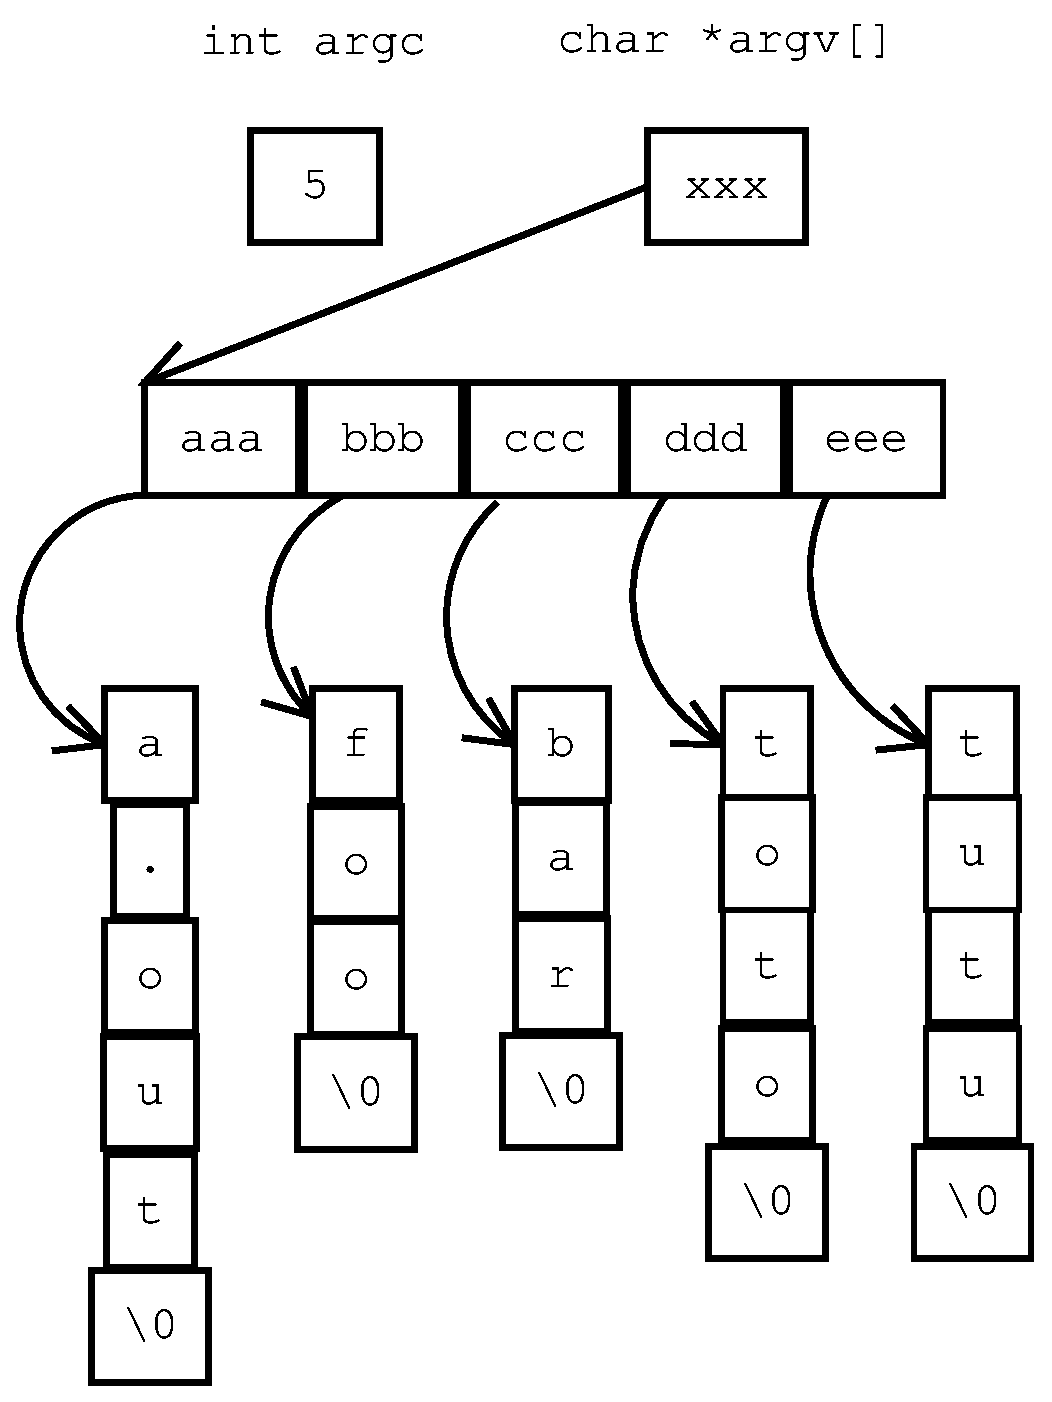
\includegraphics[scale=.35]{mainArg}
 \end{center}
\end{frame}
%------------------------------------------------------------------------------
\section{Les variables d'environnement}
\begin{frame}[fragile]
\frametitle{Les variables d'environnement}%
Les variables d'environnement correspondent aux variables du Shell. Elles sont~:
\begin{itemize}
  \item stock\'ees dans la zone de donn\'ees statique~;
  \item qui est constitu\'ee d'une suite finie de cha\^\i{}nes~: \verb?<nom>=<value>?~;
  \item accessibles par la fonction {\tt getenv}~:
  \begin{tabular}[h]{l}
       \verb?#include <stdlib.h>? \\
{\tt char *getenv(const char *name)}\\
recherche dans l'environnement une cha\^\i{}ne de la \\ forme 
{\tt  name=value}
et retourne un pointeur sur \\ {\tt value} si elle est pr\'esente.\\
\end{tabular}
\end{itemize}
\par\bigskip
Mais on peut aussi y acc\'eder par les param\`etres de la fonction main.
\index{Arguments de la ligne de commande}
\index{Variables!d'environnement} \index{\verb?argc?, \verb?argv?}
\index{\verb?getenv?}
\end{frame}
%------------------------------------------------------------------------------
\begin{frame}[fragile]
  \frametitle{Forme g\'en\'erale des param\`etres de la fonction main}%
  Cette forme est~: \verb?int main(int argc, char *argv[], char **arge)?
  
  Le dernier param\`etre \verb?arge? \'etant une suite --- termin\'ees
  par null --- de cha\^\i{}nes de caract\`eres du types~:
  \verb?varname=value?.
  
  Le code suivant affiche l'ensemble des variables d'environnement
  dont il dispose~:
\begin{verbatim}
# include <stdio.h>       
int main(int argc, char *argv[], char **arge) {
   while(*arge)
      printf("%s\n",*(arge++)) ; 
  return 0;
}
\end{verbatim}
On obtient entre autre~:
\begin{verbatim}
PWD=/home/calforme/sedoglav/Enseignement/C/Cours/Sources
TERM=xterm
OSTYPE=linux
HOST=espoir.lifl.fr
\end{verbatim}
\end{frame}
%------------------------------------------------------------------------------
\end{document}
%------------------------------------------------------------------------------


\begin{frame}
    
  \section{Structure auto-r\'ef\'erente}

 D\'efinition d'objets auto-r\'ef\'erents
\begin{itemize}
  \item inclure dans la d\'efinition de l'objet des r\'ef\'erences \`a des
    objets de m\^eme type;
  \item arbres, listes, graphes, \ldots: n\oe uds r\'ef\'eren\c{c}ant d'autres
    n\oe{}uds;
  \item type r\'ecursif: arbre binaire de recherche
\begin{verbatim}
struct noeud {
   int value;
   struct noeud *gauche, *droit;
};
\end{verbatim}
  \item place r\'eserv\'ee pour un {\em pointeur} sur une structure {\tt noeud}; \\
    \begin{bf}
        Ne r\'eserve pas de place pour stocker un objet de type {\tt
        noeud}. Pas de structure ``r\'ecursive''.
    \end{bf}
\end{itemize}

 D\'efinition d'objets en r\'ef\'erence crois\'ee
\begin{verbatim}
  struct s {                  struct t {        
    ...                         ...             
    struct t *p_t;              struct s *p_s;  
  };                          }                 
\end{verbatim}

\index{Structures!auto-r\'ef\'erentes}

\end{frame}

\begin{frame}
    
  \section{Arbre binaire de recherche}

 Programme qui affiche ses arguments tri\'es
\begin{itemize}
  \item option {\tt -r}: d\'ecroissant;
  \item Fichier {\tt abr.h}
{\normalsize
\begin{verbatim}
   typedef struct noeud {
             int v ;
             struct noeud *fg, *fd ;
           } Noeud, *Abr;

   void init(Abr *a);
   void inserer(Abr *a, int v);
   void imprimer_croissant(Abr a);
   void imprimer_decroissant(Abr a);
\end{verbatim}
}
\newpage
 \item Fichier {\tt main.c}
{\normalsize
\begin{verbatim}
   #include "abr.h"

   int main(int argc, char *argv[]) {
     char order = 0;
     Abr a;

     if (!(strcmp(argv[1], "-r"))) {
       order=1;
       argc-=1; argv+=1;
     }
     init(&a);
     while (--argc) inserer(&a, atoi(*++argv));
     if (order)
       imprimer_decroissant(a);
     else
       imprimer_croissant(a);
   }
\end{verbatim}
}

\end{itemize}

\index{Arbre binaire de recherche}

\end{frame}

\begin{frame}
    
  \section{Arbre binaire de recherche}

\begin{itemize}
  \item Fichier {\tt abr.c}
{\normalsize
\begin{verbatim}
#include "abr.h"
                              
void init (Abr *a)            void imprimer_croissant (Abr a){
 {                                if (a) {                             
   *a = NULL ;                      imprimer_croissant (a->fg) ;      
}                                   printf ("%d\n", a->v) ;           
                                    imprimer_croissant (a->fd) ;      
                                 }                                    
void inserer (Abr *a, int v)  }                                       
{
   if (! *a) {
      *a = (Abr) malloc (sizeof (struct noeud)) ;
      (*a)->v = v ;
      (*a)->fg = (*a)->fd = 0 ;
   } else if (v <= (*a)->v)
      inserer (& (*a)->fg, v) ;
   else
      inserer (& (*a)->fd, v) ;
}
\end{verbatim}
}
\end{itemize}

\index{Arbre binaire de recherche}

\end{frame}

\begin{frame}
    \section{Arbre binaire: insertion it\'erative}
    \begin{itemize}
      \item Insertion it\'erative dans l'arbre
{\normalsize
\begin{verbatim}

#define allouernoeud (struct noeud *)malloc(sizeof(struct noeud))

void inserer_iter(ABR *a, int v) {
enum {doite, gauche} direction;
ABR pere = NULL, current = *a;

while (current) {
  pere = current;
  if (v <= current->v) {
    dir = gauche;
    current = current->fg;
  } else {
    dir = droite;
    current = currrent->fd;
  }


  if (pere) 
    if (dir == gauche)
      current = pere->fg = allouer ;
    else
      current = pere->fd = allouer ;
  else
      current = *a = allouer ;
  current->v = v;
  current->fg = current->fd = NULL;
}
\end{verbatim}
}
    \end{itemize}

\index{Arbre binaire de recherche}
\end{frame}

